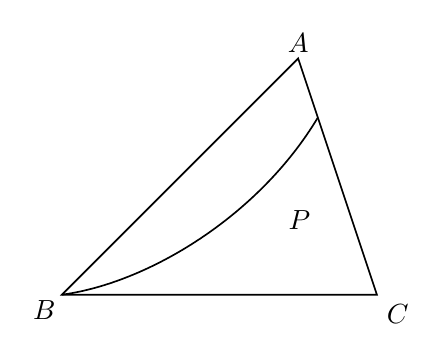
\begin{tikzpicture}[x=1cm,y=1cm,line width=.6pt,font=\normalsize]
\coordinate (L) at (0,0);
\coordinate (R) at (4,0);
\coordinate (T) at (3,3);
\coordinate (Q) at (3.25,2.25);
\draw (L)--(R)--(T)--cycle;
\draw (L) .. controls (1.1,.15) and (2.5,1.0) .. (Q);
\node[below right] at (R) {$C$};
\node[right] at (2.75,0.95) {$P$};
\node[above,inner sep=2pt] at (T) {$A$};
\node[below left,inner sep=2pt] at (L) {$B$};
\end{tikzpicture}
